\section{Resultados}

El primer experimento se realiz\'o utilizando una lista de 27 p\'aginas web, las cuales devolvieron un
total de 26 links (tan solo 12 de ellas dieron una cantidad positiva de links entrantes).

\subsection{Propagaci\'on del error}

El experimento fue realizado variando la constante c, la cual determina la importancia proporcional que se quiere
entre la probabilidad de pasar a una p\'agina desde un link (c mas alto) contra la de escribir la url a mano (c mas bajo).

El criterio de parada es la diferencia de norma uno entre el autovector que se obtiene
en cada iteraci\'on y el de la iteraci\'on anterior, el cual no debe ser menor que un
epsilon de orden -15.

\begin{figure}[H]
  \centering
    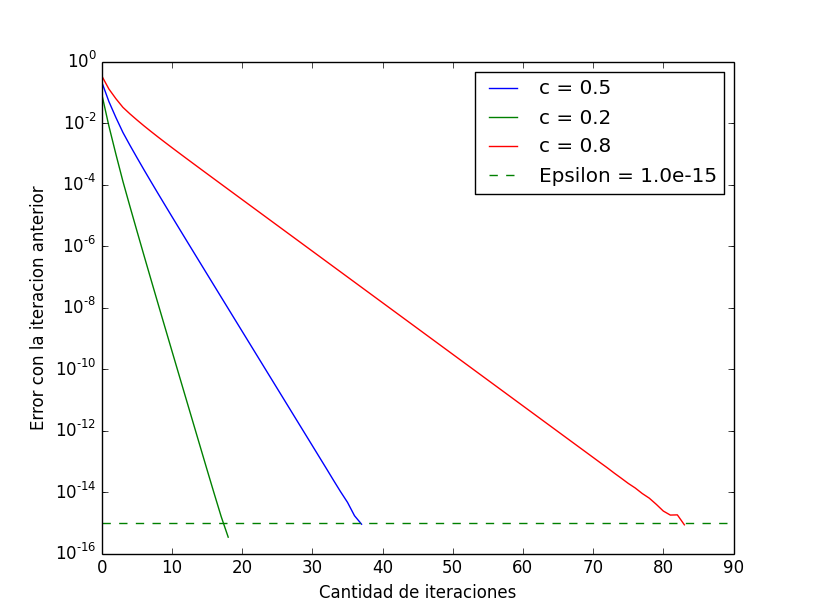
\includegraphics[width=0.9\textwidth]{../parser/graficoError1.png}
    \caption{}
    \label{}
\end{figure}

Se puede obvservar en la figura que cuanto menor es el c, m\'as r\'apido converge
el m\'etodo. Creemos que dicho resultado se debe a que al darle menor importancia
a los links directos, la matriz de probabilidades se encuentra mejor balanceada, 
por lo tanto los primeros autovalores de ella son mas parecidos y por ello se necesitan
m\'as iteraciones para lograr la convergencia. De hecho, se prob\'o bajar mas el epsilon,
el resultado fue que el m\'etodo se estabiliza en pocos pasos m\'as de los que muestra el gr\'afico,
para cada l\'inea, dejando un error igual a 0.

\subsection{Relevancia de las p\'aginas}

La relevancia siguiente fue la dada por c = 0.5 (con los otros c cambiaban un poco el orden de las p\'aginas del medio, pero 
las de mayor y menor relevancia se manten\'an igual):

\begin{tabular}{ l | c }
  \hline
  www.ole.com.ar & 0.0676399\\	
  www.clarin.com & 0.0622717\\
  www.clasificados.clarin.com & 0.0507299\\
  www.ciudad.com.ar & 0.0507299\\
  www.lanacion.com.ar/ & 0.0474195\\
  canchallena.lanacion.com.ar & 0.0474195\\
  www.rollingstone.com.ar & 0.0442582\\
  www.zonaprop.com.ar & 0.0442582\\
  www.hotmail.com & 0.0440196\\
  www.youtube.com & 0.0426776\\
  www.clarin.com/deportes & 0.0362357\\
  www.twitter.com & 0.0355646\\
  www.google.com & 0.0284517\\
  www.infobae.com & 0.0284517\\
  www.mamapuntocero.com.ar & 0.0284517\\
  www.pagina12.com.ar & 0.0284517\\
  www.yahoo.com & 0.0284517\\
  www.taringa.net & 0.0284517\\
  www.mercadolibre.com.ar & 0.0284517\\
  www.netbeans.com & 0.0284517\\
  www.github.com & 0.0284517\\
  www.assembla.com & 0.0284517\\
  www.gmail.com & 0.0284517\\
  www.9gag.com & 0.0284517\\
  www.twitter.com & 0.0284517\\
  maps.google.com.ar & 0.0284517\\
  www.stackoverflow.com & 0.0284517\\
  \hline
\end{tabular}\newline


Tal como esper\'abamos ver, las 15 p\'aginas que antes hab\'iamos notado que no ten\'ian links entrantes, son las \'ultimas
en la tabla, y no casualmente, tienen todas la misma relevancia.

Otra cosa que notamos al ir aumentando el c es que, dejando de lados los cambios en el orden de la tabla (que eran menores),
los n\'umeros cada vez se parec\'ian m\'as, ya que al darle mas importancia a las url que a los links, la cantidad
de links de entrada que posee una p\'agina no entra tanto en juego y todas se consideran iguales en t\'erminos de relevancia.

